\documentclass[12pt]{report}
\usepackage{listings}
\usepackage[table]{xcolor}
\usepackage{tabularx}
\usepackage{ltablex}
\usepackage{soul}
\sethlcolor{black!10}
\usepackage{ulem}
\usepackage{pdfpages}
\usepackage{hyperref}
\usepackage{array}
\usepackage[italian]{babel}
\usepackage[utf8]{inputenc}
\usepackage{graphicx}
\graphicspath{{images/}}
\usepackage[a4paper,width=150mm,top=15mm,bottom=15mm]{geometry}
\usepackage{fancyhdr}
\pagestyle{fancy}
\fancyhead{}
\fancyhead[L]{SavingMoneyUnina}
\fancyfoot{}
\fancyfoot[L]{pag. \thepage}
\fancyfoot[R]{\nouppercase{\leftmark}}
\renewcommand{\headrulewidth}{0.4pt}
\renewcommand{\footrulewidth}{0.4pt}
\hypersetup{colorlinks=true, linkcolor=black}

\lstset{
    language=SQL,
    basicstyle=\ttfamily,
    keywordstyle=\color{blue}\ttfamily,
    stringstyle=\color{red}\ttfamily,
    commentstyle=\color{green}\ttfamily,
    morecomment=[l][\color{magenta}]{\#},
    breaklines=true,
    postbreak=\mbox{\space},
    linewidth=\textwidth,
    escapeinside={(*@}{@*)}
}

\fancypagestyle{plain}{
    \fancyhf{}
    \renewcommand{\footrulewidth}{0.4pt}
    \fancyfoot[L]{pag. \thepage}
    \fancyfoot[R]{\nouppercase{\leftmark}}
    \renewcommand{\headrulewidth}{0mm}
}

\begin{document}

%Titlepage
\begin{titlepage} %crea l'enviroment
    \begin{figure}[t] %inserisce le figure
        \centering
\includegraphics[width=0.65\textwidth]{images/FII_logo.png}
    \end{figure}
    \vspace{20mm}
    
    \begin{Large}
     \begin{center}
        \textbf{Dipartimento di Ingegneria\\ Corso di Laurea Triennale in Informatica\\}
        \vspace{20mm}
        {\huge{\bf Progettazione e sviluppo del software SavingMoneyUnina}}\\
    \end{center}
    \end{Large}
    
    
    \vspace{36mm}
    %minipage divide la pagina in due sezioni settabili
    \begin{minipage}[t]{0.47\textwidth}
        {\large{\bf Docente:\\ Prof. Sergio Di Martino}}
    \end{minipage}
    \hfill
    \begin{minipage}[t]{0.47\textwidth}\raggedleft
        {\large{\bf Autori: \\ Francesco Donnarumma\\ N86004658\\ Arturo Donnarumma\\ N86004837\\}}
    \end{minipage}
    
    \vspace{25mm}
    
    \hrulefill
    
    \vspace{5mm}
    
    \centering{\large{\bf Anno Accademico 2023/2024 }}
    
    \end{titlepage}

\tableofcontents

%Chapter 1: Introduzione
\chapter{Introduzione}

Reprehenderit sit et ut nostrud ea adipisicing officia enim laborum fugiat veniam ad. Amet nisi ipsum nulla quis exercitation. Enim sint ex tempor cupidatat in exercitation dolore occaecat.

%Chapter 2: Class Diagram
\chapter{Progettazione Concettuale}

\section{Diagramma Delle Classi UML}

\begin{figure}[!h]
    \centering
    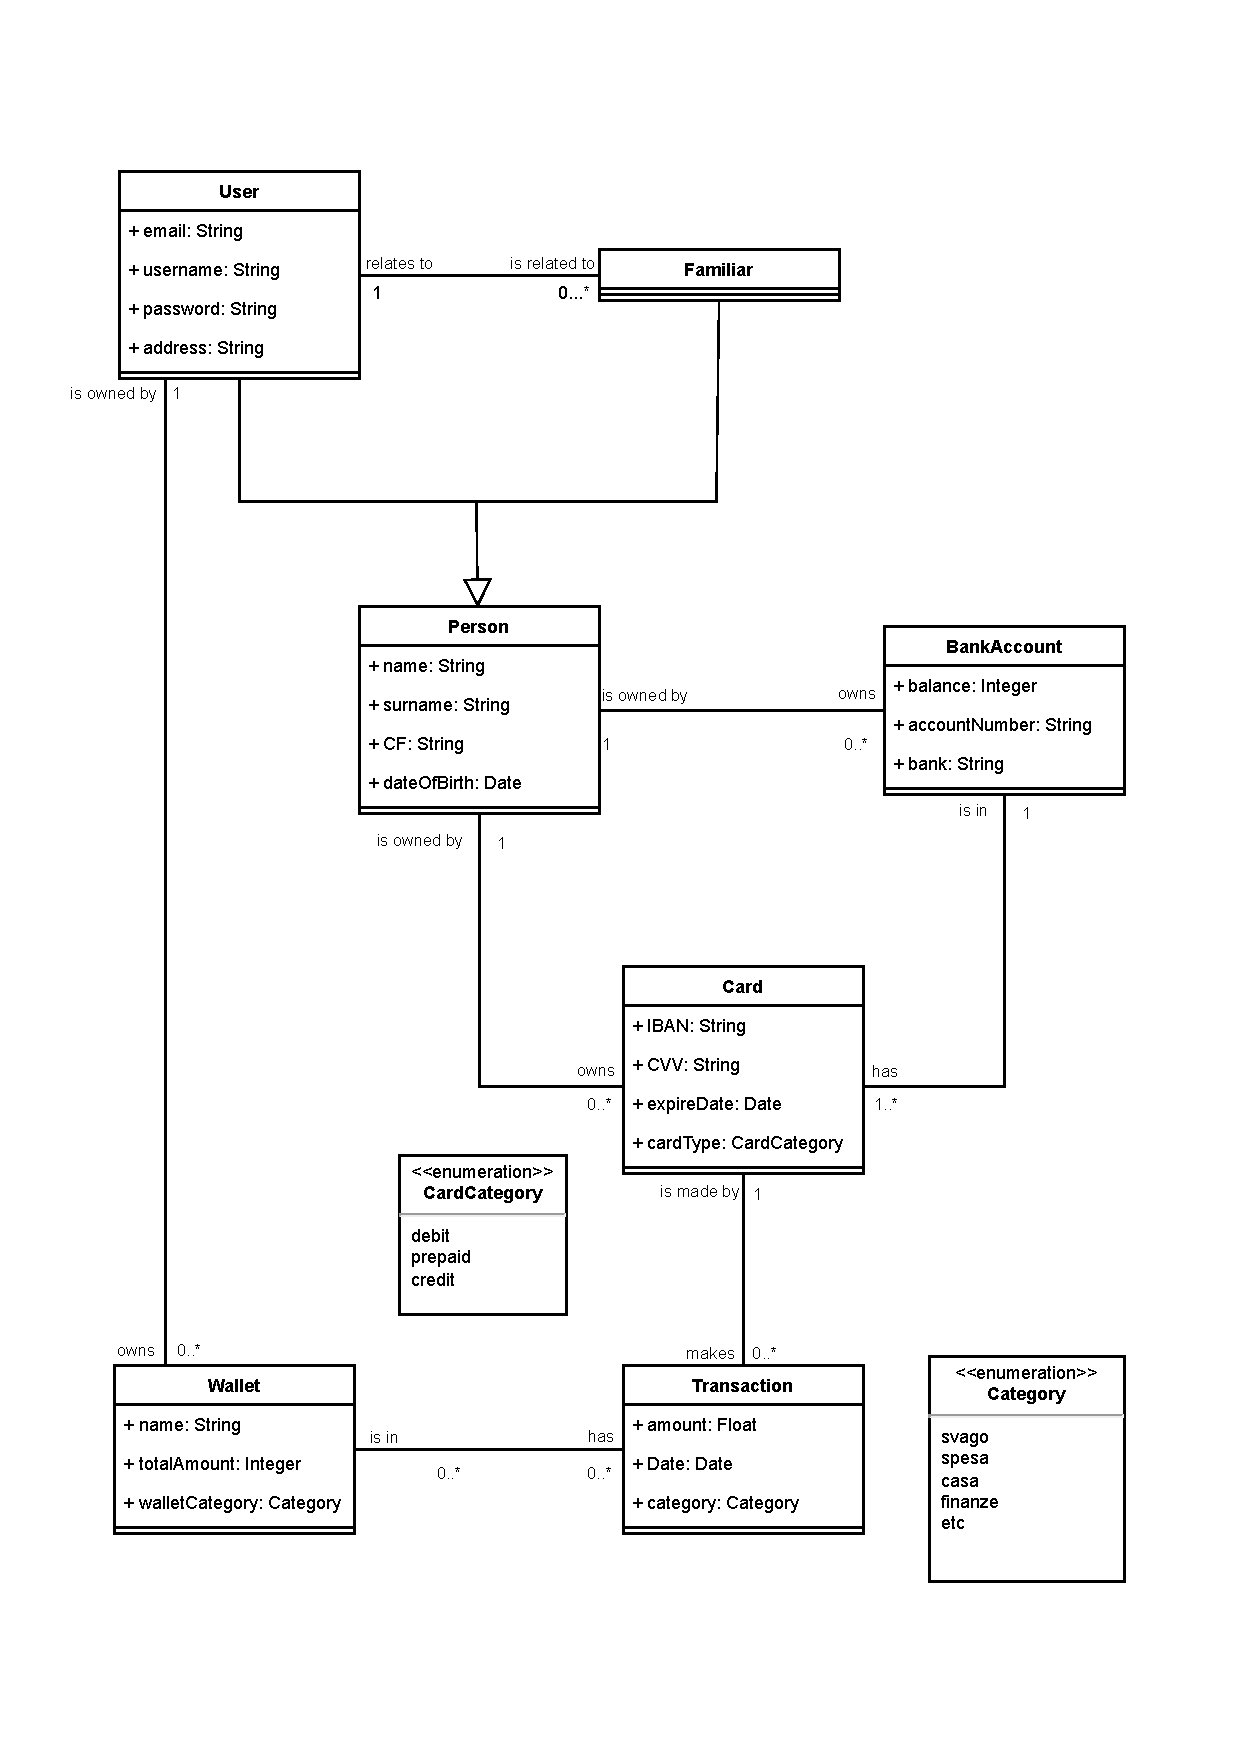
\includegraphics[scale=0.55]{pdfs/UMLdiagram.drawio.pdf}
    \caption{Diagramma UML}\label{UML}
\end{figure}

\section{Diagramma ER (Entità Relazione)}

\begin{figure}[!h]
    \centering
    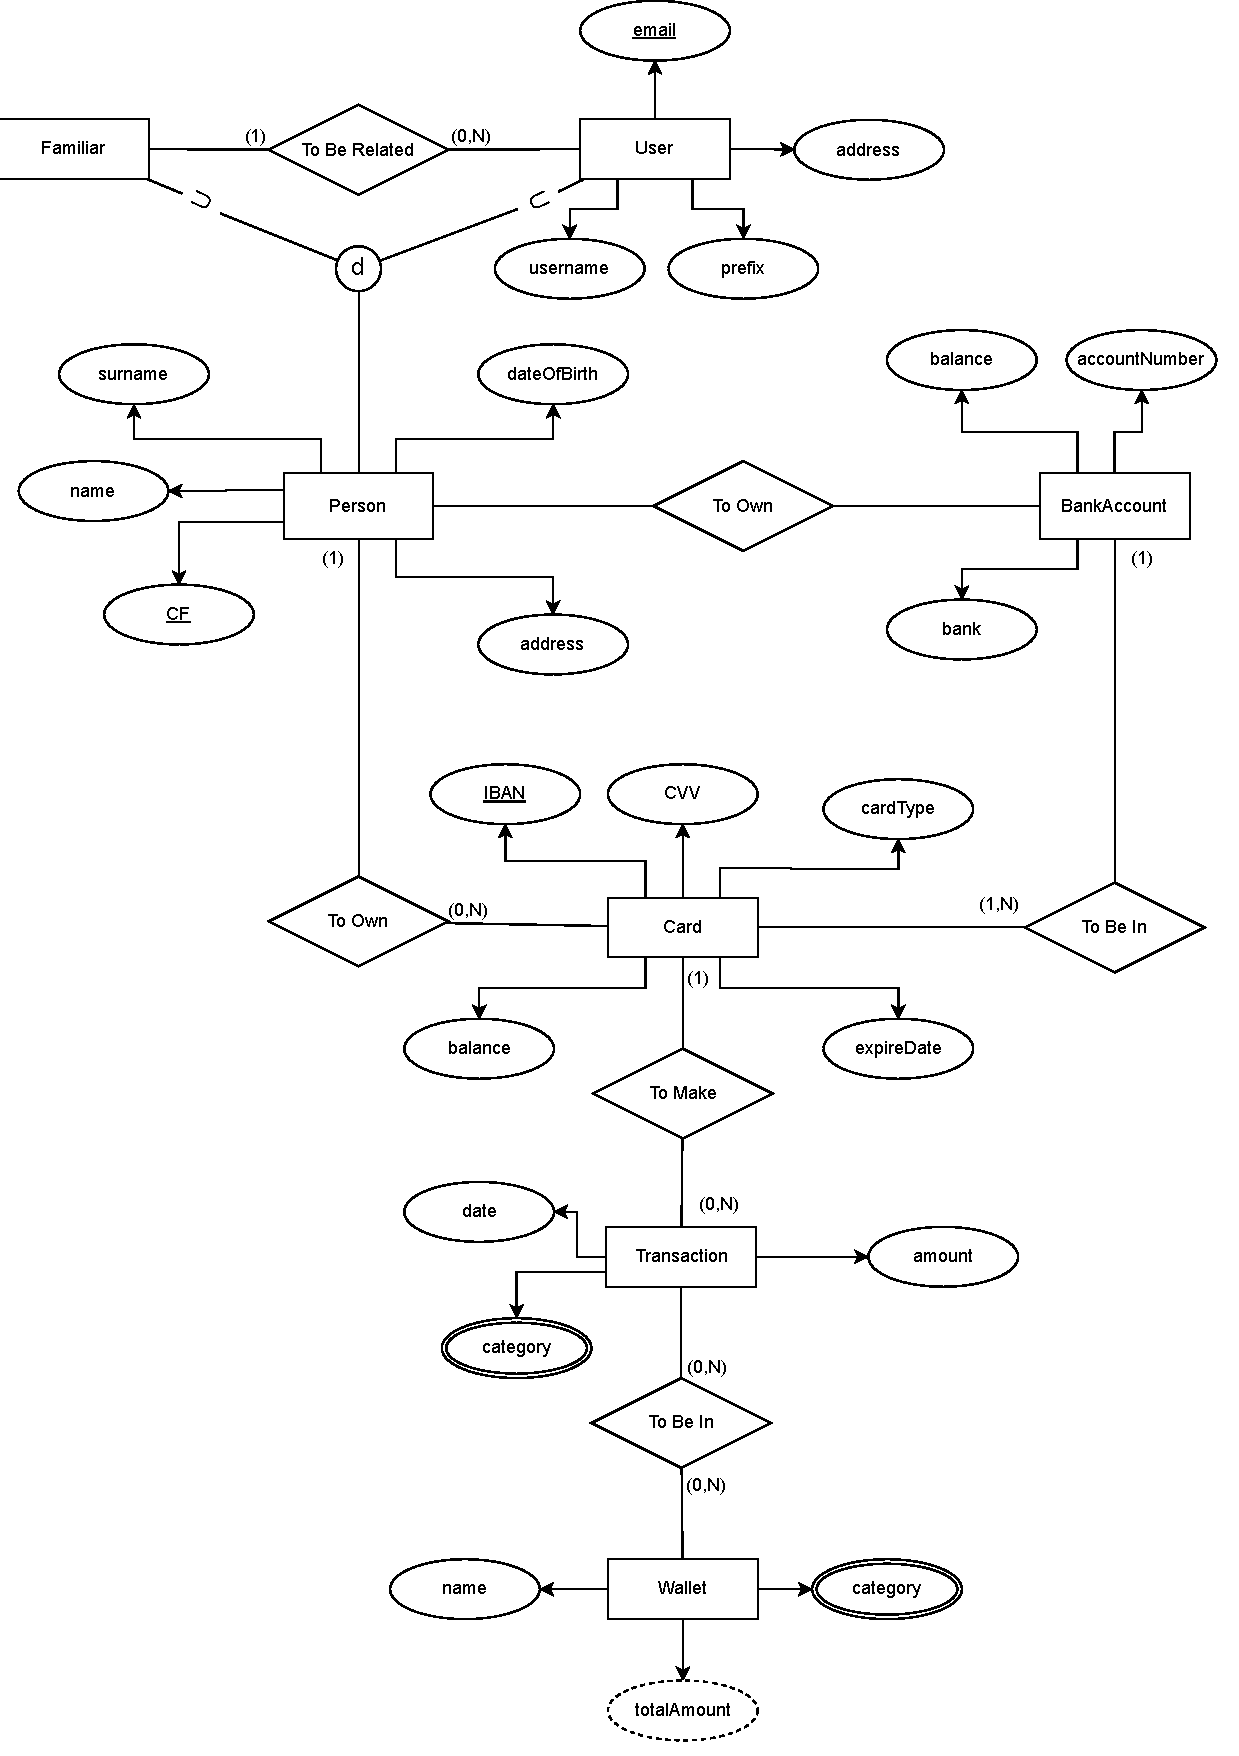
\includegraphics[scale=0.7]{pdfs/ERdiagram.drawio.pdf}
    \caption{Diagramma ER}\label{ER}
\end{figure}

\newpage

\section{Ristrutturazione}

\subsection{Attributi multipli}

Per quanto riguarda la gestione di attributi multipli,
abbiamo deciso di gestire l'attributo \textit{category} della tabella
\textbf{Transaction}, originariamente definito come enumerazione,
trasformandolo in una stringa, poiché non abbiamo bisogno di valori
specifici, trattandosi di una categoria personalizzabile.

Anche per l'attributo \textit{cardType} è stata applicata la stessa
procedura. Il controllo dell'attributo verrà gestito tramite i vincoli
approfonditi nel dizionario dei vincoli.

\subsection{Generalizzazioni}

Per la generalizzazione, essendo di tipologia totale e disgiunta,
abbiamo optato per il metodo di eliminare la classe generale.
Abbiamo trasferito tutti gli attributi di essa nelle
classi specializzate, conservando le relative relazioni.

\subsection{Analisi degli identificativi}

Per la maggior parte delle classi, saranno utilizzati come identificativi
attributi già presenti di natura nelle classi stesse, poiché risultano
sufficienti e non richiedono l'uso di una chiave surrogata.
Tuttavia, in alcune classi, sono presenti chiavi surrogate,
identificate con il prefisso \textbf{ID\_}.

\newpage
\subsection{Diagramma UML ristrutturato}

\begin{figure}[!h]
    \centering
    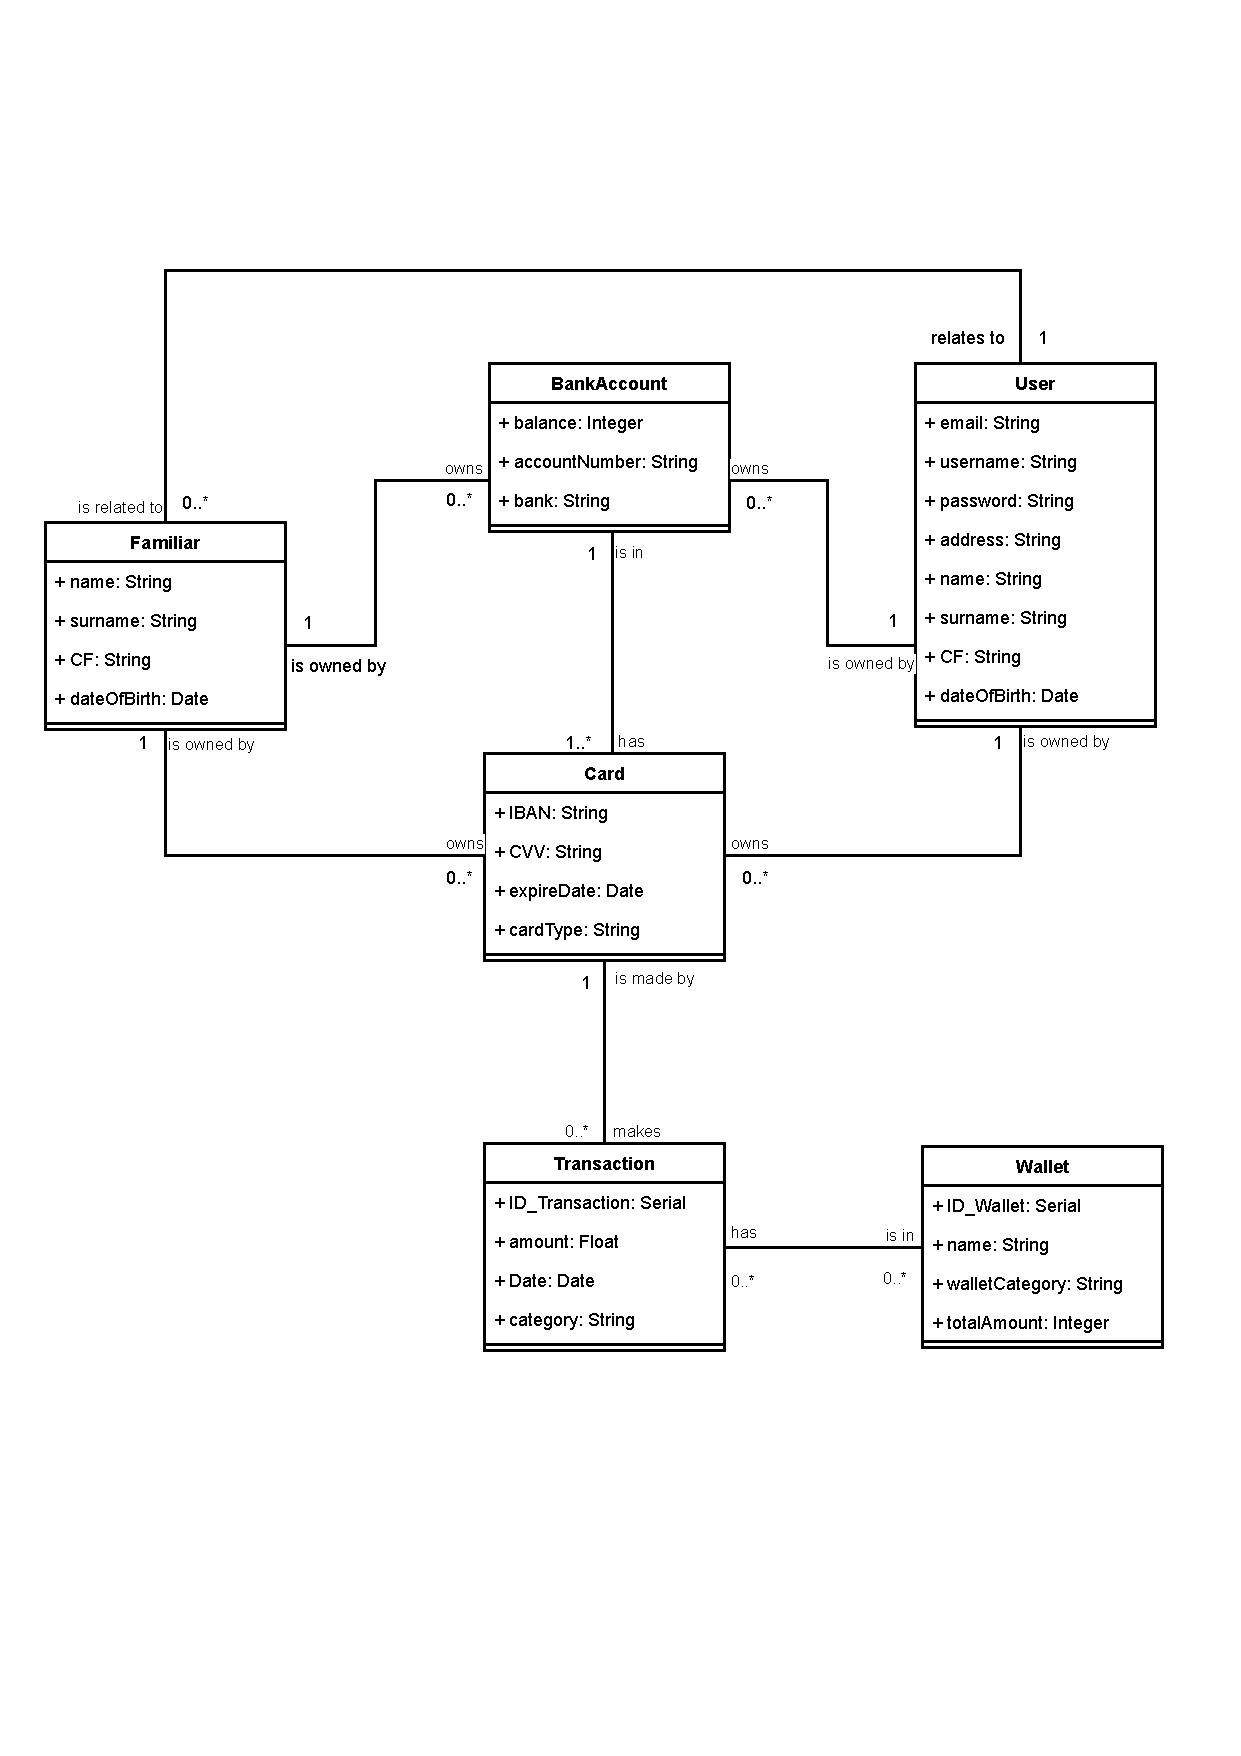
\includegraphics[scale=0.7]{pdfs/RestructuredUMLdiagram.drawio.pdf}
    \caption{Diagramma UML Ristrutturato}\label{ResUML}
\end{figure}

\newpage
\section{Dizionari}

\subsection{Dizionario delle classi}

\begin{longtable}{m{2.7cm}|m{4cm}|m{7cm}}

    \rowcolor{black!10}
    \textbf{Classe} & \textbf{Descrizione} & \textbf{Attributi} \\ \hline
    \endhead

    \textbf{User} & \raggedright Classe utilizzata per identificare gli utenti registrati alla piattaforma. &
    \parbox{7cm}{
        \textbf{email} (\textit{String}): chiave primaria, email con la quale l'utente si è registrato. \\ 
        \textbf{username} (\textit{String}): nome che viene mostrato per riconoscere lo stesso. \\
        \textbf{password} (\textit{String}): stringa atta alla convalidazione durante l'accesso all'account. \\
        \textbf{address} (\textit{String}): indirizzo del domicilio. \\
        \textbf{name} (\textit{String}): nome. \\
        \textbf{surname} (\textit{String}): cognome. \\
        \textbf{CF} (\textit{String}): codice fiscale. \\
        \textbf{dateOfBirth} (\textit{Date}): data di nascita.
    } \\ \hline

    \textbf{Familiar} & \raggedright Classe utilizzata per identificare i familiari degli utenti presenti nel database. &
    \parbox{7cm}{
        \textbf{name} (\textit{String}): nome. \\
        \textbf{surname} (\textit{String}): cognome. \\
        \textbf{CF} (\textit{String}): codice fiscale, chiave primaria nel caso del familiare. \\
        \textbf{dateOfBirth} (\textit{Date}): data di nascita.
    } \\ \hline

    \textbf{BankAccount} & \raggedright Classe utilizzata per identificare i conti correnti appartenenti a utenti o familiari. &
    \parbox{7cm}{
        \textbf{balance} (\textit{Integer}): indica il saldo disponibile sul conto corrente. \\
        \textbf{accountNumber} (\textit{String}): chiave primaria, identificativa del conto corrente. \\
        \textbf{bank} (\textit{String}): nome della banca alla quale è associato il conto corrente.
    } \\ \hline

    \textbf{Card} & \raggedright Classe utilizzata per identificare le carte appartenenti a utenti o familiari. &
    \parbox{7cm}{
        \textbf{IBAN} (\textit{String}): codice identificativo della carta. \\
        \textbf{CVV} (\textit{String}): codice di sicurezza per le transazioni delle carte. \\
        \textbf{expireDate} (\textit{Date}): data che indica la scadenza della carta. \\
        \textbf{cardType} (\textit{String}): campo che indica la tipologia della carta.
    } \\ \hline

    \textbf{Transaction} & \raggedright Classe utilizzata per tenere traccia di tutte le transazioni effettuate. &
    \parbox{7cm}{
        \textbf{ID\_Transaction} (\textit{Serial}): chiave surrogata, identificativo della singola transazione. \\
        \textbf{amount} (\textit{Float}): indica l'ammontare della transazione. \\
        \textbf{date} (\textit{Date}): data in cui è avvenuta la transazione. \\
        \textbf{category} (\textit{String}): tipologia di transazione. Serve per l'associazione automatica ai portafogli.
    } \\ \hline

    \textbf{Wallet} & \raggedright Classe utilizzata per raggruppare transazioni. &
    \parbox{7cm}{
        \textbf{ID\_Wallet} (\textit{Serial}): chiave surrogata, identificativo del singolo protafoglio. \\
        \textbf{name} (\textit{String}): nome del portafoglio. \\
        \textbf{walletCategory} (\textit{String}): categoria del portafoglio. \\
        \textbf{totalAmount} (\textit{Float}): indica la somma di tutte le transazioni relative al portafoglio.
    } \\ \hline

\end{longtable}

\subsection{Dizionario delle associazioni}

\begin{longtable}{m{2.7cm}|m{4cm}|m{7cm}}
    
    \rowcolor{black!10}
    \textbf{Associazione} & \textbf{Descrizione} & \textbf{Classi coinvolte} \\ \hline
    \endhead

    \raggedright \textbf{To Be Related} & \raggedright Esprime la parentela tra gli utenti e i familiari &
    \parbox{7cm}{
        \textbf{Familiar [1]} (\textbf{relates to}): indica, per ogni familiare, con quale utente è imparentato. \\
        \textbf{User [0..*]} (\textbf{is related to}): indica quali sono i familiari che sono imparentati con esso.
    } \\ \hline

    \raggedright \textbf{To Own} & \raggedright Esprime il possesso degli utenti sui conti correnti &
    \parbox{7cm}{
        \textbf{User [0..*]} (\textbf{owns}): indica, per ogni utente, quali sono i conti correnti che possiede. \\
        \textbf{BankAccount [1]} (\textbf{is owned by}): indica l'utente che possiede il conto corrente in questione.
    } \\ \hline

    \raggedright \textbf{To Own} & \raggedright Esprime il possesso dei familiari sui conti correnti &
    \parbox{7cm}{
        \textbf{Familiar [0..*]} (\textbf{owns}): indica, per ogni familiare, quali sono i conti correnti che possiede. \\
        \textbf{BankAccount [1]} (\textbf{is owned by}): indica il familiare che possiede il conto corrente in questione.
    } \\ \hline

    \raggedright \textbf{To Be In} & \raggedright Esprime la correlazione tra le carte e i conti correnti &
    \parbox{7cm}{
        \textbf{Card [1]} (\textbf{is in}): indica, per ogni carta, qual è il conto corrente a cui sono associate. \\
        \textbf{BankAccount [1..*]} (\textbf{has}): indica quali sono le carte che sono associate al conto corrente in questione.
    } \\ \hline

    \raggedright \textbf{To Own} & \raggedright Esprime il possesso degli utenti sulle carte &
    \parbox{7cm}{
        \textbf{User [0..*]} (\textbf{owns}): indica, per ogni utente, quali sono le carte che possiede. \\
        \textbf{Card [1]} (\textbf{is owned by}): indica l'utente che possiede la carta in questione.
    } \\ \hline

    \raggedright \textbf{To Own} & \raggedright Esprime il possesso dei familiari sulle carte &
    \parbox{7cm}{
        \textbf{Familiar [0..*]} (\textbf{owns}): indica, per ogni utente, quali sono le carte che possiede. \\
        \textbf{Card [1]} (\textbf{is owned by}): indica l'utente che possiede la carta in questione.
    } \\ \hline

    \raggedright \textbf{To Make} & \raggedright Esprime il collegamento una la transazione e la carta con la quale è stata effettuata &
    \parbox{7cm}{
        \textbf{Card [0..*]} (\textbf{makes}): indica, per ogni carta, tutte le transazioni effettuate. \\
        \textbf{Transaction [1]} (\textbf{is made by}): indica con quale carta è stata effettuata la transazione in questione.
    } \\ \hline

    \raggedright \textbf{To Be In} & \raggedright Esprime la correlazione tra le transazioni e i portafogli &
    \parbox{7cm}{
        \textbf{Wallet [0..*]} (\textbf{has}): indica, per ogni portafoglio, quali sono le transazioni che lo compongono. \\
        \textbf{Transaction [0..*]} (\textbf{is in}): indica qual è il portafoglio a cui fa riferimento la transazione in questione.
    } \\ \hline

\end{longtable}

\subsection{Dizionario dei vincoli}

\begin{longtable}{m{5.2cm}|m{2.8cm}|m{5.3cm}}
    
    \rowcolor{black!10}
    \textbf{Vincolo} & \textbf{Tipo} & \textbf{Descrizione} \\ \hline
    \endhead

    \raggedright \textbf{unique\_username} & \raggedright Intrarelazionale &
    Nella tabella User non ci possono essere t-uple diverse con lo stesso username. \\ \hline

    \raggedright \textbf{unique\_CF} & \raggedright Intrarelazionale &
    Nella tabella User non ci possono essere t-uple diverse con lo stesso CF. \\ \hline

    \raggedright \textbf{check\_BirthDate\_User} & \raggedright Dominio &
    Nella tabella User la data deve essere necessariamente antecedente alla data odierna. \\ \hline

    \raggedright \textbf{check\_BirthDate\_Familiar} & \raggedright Dominio &
    Nella tabella Familiar la data deve essere necessariamente antecedente alla data odierna. \\ \hline

    \raggedright \textbf{ownership\_check\_BA} & \raggedright N-upla &
    Per ogni t-upla della tabella BankAccount, essa deve essere associata necessariamente o ad un Utente o ad un Familiare, ma non ad entrambi. \\ \hline

    \raggedright \textbf{ownership\_check\_Card} & \raggedright N-upla &
    Per ogni t-upla della tabella Card, essa deve essere associata necessariamente o ad un Utente o ad un Familiare, ma non ad entrambi. \\ \hline

    \raggedright \textbf{cardType\_Check} & \raggedright Dominio &
    Nella tabella Card, per ogni t-upla, il campo cardCategory deve essere necessariamente “prepaid”, “debit” o “credit”. \\ \hline

    \raggedright \textbf{check\_Transaction\_Date} & \raggedright Dominio &
    Nella tabella Transaction, per ogni t-upla, la data deve essere necessariamente antecedente o coincidente alla data odierna. \\ \hline

\end{longtable}

%Chapter 3: Sequence Diagrams
\chapter{Ristrutturazione}



%Chapter 4: Conclusione
\chapter{Schema Fisico}

\section{Definizoni SQL delle tabelle}

\subsection{User}

\begin{lstlisting}
CREATE TABLE smu."user"(*@\footnote{vengono usate le virgolette perche' altrimenti la parola \textit{user} verrebbe identificata come keyword}@*) (
    email character varying(100) NOT NULL,
    username character varying(20) NOT NULL,
    password character varying(30) NOT NULL,
    address character varying(100),
    name character varying(20) NOT NULL,
    surname character varying(30) NOT NULL,
    cf character varying(16) NOT NULL,
    dateofbirth date NOT NULL,
    CONSTRAINT check_birthdate_user CHECK ((dateofbirth < CURRENT_DATE))
);
\end{lstlisting}

\subsection{Familiar}

\begin{lstlisting}
CREATE TABLE smu.familiar (
    name character varying(20) NOT NULL,
    surname character varying(30) NOT NULL,
    cf character varying(16) NOT NULL,
    dateofbirth date NOT NULL,
    familiaremail character varying(100) NOT NULL,
    CONSTRAINT check_birthdate_familiar CHECK ((dateofbirth < CURRENT_DATE))
);
\end{lstlisting}

\newpage

\subsection{BankAccount}

\begin{lstlisting}
CREATE TABLE smu.bankaccount (
    balance integer NOT NULL,
    accountnumber integer NOT NULL,
    bank character varying(40),
    ownercf character varying(16),
    owneremail character varying(100),
    CONSTRAINT ownership_check_ba CHECK (((ownercf IS NULL) <> (owneremail IS NULL)))
);
\end{lstlisting}

\subsection{Card}

\begin{lstlisting}
CREATE TABLE smu.card (
    cardnumber character varying(16) NOT NULL,
    iban character varying(27) NOT NULL,
    cvv character varying(3) NOT NULL,
    expiredata date NOT NULL,
    cardtype character varying(11),
    ba_number integer NOT NULL,
    ownercf character varying(16),
    owneremail character varying(100),
    CONSTRAINT cardtype_check CHECK (((cardtype)::text = ANY (ARRAY[('Prepagata'::character varying)::text, ('Debito'::character varying)::text, ('Credito'::character varying)::text]))),
    CONSTRAINT ownership_check_card CHECK (((ownercf IS NULL) <> (owneremail IS NULL)))
);
\end{lstlisting}

\subsection{Transaction}

\begin{lstlisting}
CREATE TABLE smu.transaction (
    id_transaction integer NOT NULL,
    amount double precision NOT NULL,
    date date NOT NULL,
    category character varying(35),
    cardnumber character varying(16) NOT NULL,
    walletname character varying(35),
    CONSTRAINT check_transaction_date CHECK ((date <= CURRENT_DATE))
);
\end{lstlisting}

\subsection{Wallet}

\begin{lstlisting}
CREATE TABLE smu.wallet (
    id_wallet integer NOT NULL,
    walletname character varying(35) NOT NULL,
    walletcategory character varying(35) NOT NULL,
    totalamount double precision NOT NULL,
    owneremail character varying(100) NOT NULL
);
\end{lstlisting}

\subsection{TransactionInWallet}

\begin{lstlisting}
CREATE TABLE smu.transactioninwallet (
    id_transaction integer NOT NULL,
    id_wallet integer NOT NULL
);
\end{lstlisting}

\section{Definizoni SQL dei trigger}

\subsection{check\_card\_owner\_trigger}

\begin{lstlisting}
CREATE TRIGGER check_card_owner_trigger
    BEFORE INSERT ON smu.card
    FOR EACH ROW
    EXECUTE FUNCTION smu.check_card_owner();
\end{lstlisting}

\begin{lstlisting}
    CREATE FUNCTION smu.check_card_owner() RETURNS trigger
    LANGUAGE plpgsql
    AS $$
DECLARE
    BA_used smu.bankaccount%ROWTYPE;
    familiar_email smu.familiar.familiaremail%TYPE;
BEGIN

    familiar_email := NULL;

    -- Recupera le informazioni relative al conto corrente
    -- al quale si sta associando la carta
    SELECT *
    INTO BA_used
    FROM smu.bankaccount
    WHERE accountnumber = NEW.ba_number;

    -- Recupera l'email dell'account al quale e' associato
    -- il familiare, proprietario della carta
    IF NEW.ownercf IS NOT NULL THEN
        SELECT familiaremail
        INTO familiar_email
        FROM smu.familiar
        WHERE cf = NEW.ownercf;
    END IF;

    -- Se tutte le condizioni sono vere, viene inserita la carta, altrimenti viene restituita una exception
    IF (BA_used.owneremail = NEW.owneremail OR BA_used.ownercf = NEW.ownercf) OR
    (familiar_email = BA_used.owneremail) OR BA_used.ownercf IN (SELECT CF FROM smu.familiar WHERE familiaremail = NEW.owneremail)
    THEN
        -- L'IF e' stato strutturato in questo modo perche' non basta negare le condizioni per avere
        -- solo un IF THEN. Questo perche' nel caso in cui alcuni attributi sono NULL il sistema
        -- non e' in grado di fornire una valutazione sulla condizione, quindi gli AND da sostituire
        -- agli attuali OR sarebbero sempre falsi.
    ELSE
        RAISE EXCEPTION 'Il proprietario della carta deve essere anche il proprietario del conto corrente, o al massimo un suo familiare.';
    END IF;

    -- Nell'ultima porzione della condizione dell'IF viene controllato se il codice fiscale
    -- del proprietario del conto corrente e' presente nell'elenco dei familiari associati
    -- all'email del proprietario della carta

    RETURN NEW;
END;
$$;
\end{lstlisting}

\subsection{connect\_transaction\_to\_wallet\_trigger}

\begin{lstlisting}
    CREATE TRIGGER connect_transaction_to_wallet_trigger 
    AFTER INSERT OR UPDATE ON smu.transaction 
    FOR EACH ROW 
    EXECUTE FUNCTION smu.connect_transaction_to_wallet();
\end{lstlisting}

\begin{lstlisting}
    CREATE OR REPLACE FUNCTION smu.connect_transaction_to_wallet() RETURNS trigger
    LANGUAGE plpgsql
    AS $$
DECLARE
    wallet_row smu.wallet%ROWTYPE;
    card_row smu.card%ROWTYPE;
    old_card_row smu.card%ROWTYPE;
    account_email smu.user.email%TYPE;
    ba_row smu.bankaccount%ROWTYPE;
    old_ba_row smu.bankaccount%ROWTYPE;
BEGIN

    -- Seleziono la carta con la quale e' stata effettuata la transazione
    SELECT *
    INTO card_row
    FROM smu.card
    WHERE cardnumber = NEW.cardnumber;

    -- Controlla se la carta e' scaduta o meno al momento della transazione
    IF smu.expired_card(card_row.expiredata, NEW.date) THEN
        RAISE EXCEPTION 'La carta risultava scaduta al momento della transazione';
    END IF;

    -- Recupero il conto corrente al quale e' associato la carta
    SELECT *
    INTO ba_row
    FROM smu.bankaccount
    WHERE accountnumber = card_row.ba_number;
    
    -- Controllo se la transazione puo' essere effettuata o meno
    IF TG_OP = 'INSERT' AND ba_row.balance < NEW.amount THEN
        RAISE EXCEPTION 'Saldo sul conto corrente insufficiente';
    ELSIF TG_OP = 'UPDATE' AND (ba_row.balance + OLD.amount) < NEW.amount THEN
        RAISE EXCEPTION 'Saldo sul conto corrente insufficiente al momento della transazione';
    END IF;

    -- Recupero l'email dell'account al quale saranno associati i portafogli
    IF card_row.owneremail IS NOT NULL THEN
        -- Se la carta appartiene ad un utente, mi salvo l'email nella variabile account_email
        account_email := card_row.owneremail;
    ELSE
        -- Altrimenti, appartiene sicuramente ad un familiare e vado a
        -- recuperare l'email dell'utente al quale e' associato
        SELECT familiaremail
        INTO account_email
        FROM smu.familiar
        WHERE cf = card_row.ownercf;
    END IF;

    IF TG_OP = 'INSERT' THEN
        -- Trova i wallet con la stessa categoria della transazione
        -- appena inserita che appartengono all'utente corretto
		IF NEW.walletName IS NULL THEN
			FOR wallet_row IN
				SELECT *
				FROM smu.wallet
				WHERE walletcategory = NEW.category AND owneremail = account_email
			LOOP

				-- Collega la transazione al wallet trovato
				INSERT INTO smu.transactioninwallet (id_transaction, id_wallet)
				VALUES (NEW.id_transaction, wallet_row.id_wallet);

				-- Aggiorna il campo totalamount del wallet
				UPDATE smu.wallet
				SET totalamount = totalamount + NEW.amount
				WHERE id_wallet = wallet_row.id_wallet;

			END LOOP;

			-- Aggiorna il saldo del conto corrente
			UPDATE smu.bankaccount
			SET balance = balance - NEW.amount
			WHERE accountnumber = ba_row.accountnumber;
		ELSE
			FOR wallet_row IN
				SELECT *
				FROM smu.wallet
				WHERE walletcategory = NEW.category AND owneremail = account_email AND walletName = NEW.walletName
			LOOP

				-- Collega la transazione al wallet trovato
				INSERT INTO smu.transactioninwallet (id_transaction, id_wallet)
				VALUES (NEW.id_transaction, wallet_row.id_wallet);

				-- Aggiorna il campo totalamount del wallet
				UPDATE smu.wallet
				SET totalamount = totalamount + NEW.amount
				WHERE id_wallet = wallet_row.id_wallet;

			END LOOP;

			-- Aggiorna il saldo del conto corrente
			UPDATE smu.bankaccount
			SET balance = balance - NEW.amount
			WHERE accountnumber = ba_row.accountnumber;
		END IF;
    END IF;

    IF TG_OP = 'UPDATE' THEN

        -- Se e' stata modificata la categoria, la transazione viene collegata ai nuovi portafogli
        -- altrimenti viene ricollegata agli stessi

        -- Scollego la transazione da tutti i portafogli
        DELETE FROM smu.transactioninwallet WHERE id_transaction = OLD.id_transaction;
        
        -- Seleziona tutti i portafogli a cui era collegata la transazione
        FOR wallet_row IN
            SELECT *
            FROM smu.wallet
            WHERE walletcategory = OLD.category AND owneremail = account_email
        LOOP

            -- Aggiorna il campo totalamount del wallet
            UPDATE smu.wallet
            SET totalamount = totalamount - OLD.amount
            WHERE id_wallet = wallet_row.id_wallet;

        END LOOP;

        -- Seleziona tutti i portafogli a cui deve essere collegata la transazione
        FOR wallet_row IN
            SELECT *
            FROM smu.wallet
            WHERE walletcategory = NEW.category AND owneremail = account_email
        LOOP

            -- Collega la transazione al wallet trovato
            INSERT INTO smu.transactioninwallet (id_transaction, id_wallet)
            VALUES (NEW.id_transaction, wallet_row.id_wallet);

            -- Aggiorna il campo totalamount del wallet
            UPDATE smu.wallet
            SET totalamount = totalamount + NEW.amount
            WHERE id_wallet = wallet_row.id_wallet;

        END LOOP;        

        -- Seleziono la carta con la quale e' stata effettuata inizialmente la transazione
        SELECT *
        INTO old_card_row
        FROM smu.card
        WHERE iban = OLD.cardiban;

        -- Recupero il conto corrente al quale e' associato la vecchia carta
        SELECT *
        INTO old_ba_row
        FROM smu.bankaccount
        WHERE accountnumber = old_card_row.ba_number;

        -- Aggiorno il saldo del vecchio conto corrente
        UPDATE smu.bankaccount
        SET balance = balance + OLD.amount
        WHERE accountnumber = old_ba_row.accountnumber;

        -- Aggiorno il saldo del nuovo conto corrente
        UPDATE smu.bankaccount
        SET balance = balance - NEW.amount
        WHERE accountnumber = ba_row.accountnumber;

    END IF;

    RETURN NEW;
END;
$$;
\end{lstlisting}

\newpage

\subsection{update\_wallet\_category\_trigger}

\begin{lstlisting}
    CREATE TRIGGER update_wallet_category_trigger 
    AFTER UPDATE OF walletcategory ON smu.wallet 
    FOR EACH ROW 
    EXECUTE FUNCTION smu.update_wallet_category();
\end{lstlisting}

\begin{lstlisting}
CREATE FUNCTION smu.update_wallet_category() RETURNS trigger
    LANGUAGE plpgsql
    AS $$
DECLARE
    transaction_row smu.transaction%ROWTYPE;
BEGIN

    -- Vengono scollegate tutte le transazioni dal wallet
    DELETE FROM smu.transactioninwallet WHERE id_wallet = OLD.id_wallet;

    -- Reimposta a 0 la somma degli importi del portafoglio
    UPDATE smu.wallet
    SET totalamount = 0
    WHERE id_wallet = NEW.id_wallet;

    FOR transaction_row IN
        SELECT *
        FROM smu.transaction AS T
        WHERE T.category = NEW.walletcategory AND T.cardiban IN 
        (SELECT iban FROM smu.card WHERE owneremail = NEW.owneremail
        UNION SELECT C.iban
        FROM smu.familiar AS F
        JOIN smu.card AS C ON F.cf = C.ownercf
        WHERE familiaremail = NEW.owneremail)
    LOOP

        -- Collega la transazione trovata
        INSERT INTO smu.transactioninwallet (id_transaction, id_wallet)
        VALUES (transaction_row.id_transaction, NEW.id_wallet);

        -- Aggiorna il campo totalamount del wallet
        UPDATE smu.wallet
        SET totalamount = totalamount + transaction_row.amount
        WHERE id_wallet = NEW.id_wallet;

    END LOOP;

    RETURN NEW;
    
END;
$$;
\end{lstlisting}

\section{Definizoni SQL delle funzioni}

\subsection{expired\_card}

\begin{lstlisting}
    CREATE FUNCTION smu.expired_card(card_expire_date date, transaction_date date) RETURNS boolean
    LANGUAGE plpgsql
    AS $$
BEGIN
    -- Questa funzione controlla se la carta data in input era scaduta
    -- al momento della transazione data in input. La funzione viene usata
    -- all'interno della funzione "connect_transaction_to_wallet" la quale viene
    -- eseguita ad ogni inserimento di una nuova transazione.
    -- Questa funzione viene utilizzata per garantire il vincolo "check_expire_date".
    IF card_expire_date < transaction_date THEN
        RETURN TRUE;
    ELSE
        RETURN FALSE;
    END IF;
END;
$$;
\end{lstlisting}

\end{document}